% ch13-ml.tex -- Reinforcement learning
\chapter{Reinforcement learning}
\label{ch:rl}

Everything until now learned from a fixed dataset: $\{(\mathbf x_i,
y_i)\}$, predict, score, stop. This chapter breaks that frame. A
reinforcement-learning agent is not shown correct answers --- it takes
an \emph{action}, receives a \emph{reward}, and must figure out which
choices were good from delayed, partial credit. The problems this
solves have no dataset at all: game moves, control policies, robot
steps --- and the fine-tuning loops that align language models. We
build it the honest way: bandits first (the exploration problem in
isolation), then the full Markov decision process, value functions and
the Bellman equation, tabular Q-learning that actually works on a
grid, and finally function approximation --- where the theory cracks
and we let it crack on camera, because a CartPole that learns and
then unlearns is worth more than a wall of caveats.

% from-zero:begin
\begin{rulebox}[Before you start]
Chapters~7--8 and \textbf{Book~3, Chapter~12}. \emph{Recap:} so far the data were given. In reinforcement learning an agent chooses actions, and the data it sees depend on those choices.
\end{rulebox}
\begin{wins}[After this chapter you can]
\begin{itemize}
\item formulate a problem as an MDP with states, actions, rewards and a discount;
\item solve a bandit problem and explain exploration versus exploitation;
\item write the Bellman equations and run Q-learning;
\item state the policy-gradient idea in one page.
\end{itemize}
\end{wins}
\begin{principle}[How to think about this]
In reinforcement learning nobody tells you the right action; you learn from consequences, and your choices change what you see next. The central tension is exploration (try new things) against exploitation (use what works). The Bellman equation says a state's value is the reward now plus the value of where you land.
\end{principle}
% from-zero:end

\section{From prediction to action: agent, environment, reward}
\label{sec:loop}

The loop is the whole model: at each step the agent sees a
\emph{state} $s_t$, picks an \emph{action} $a_t$ from its
\emph{policy}\index{policy} $\pi$, the environment replies with a
scalar \emph{reward}\index{reward} $r_{t+1}$ and a next state
$s_{t+1}$ --- repeat. Supervised learning's ``correct answer'' is
replaced by \emph{experience}: the agent must infer good actions from
the reward stream, possibly long after the action that earned them.

\begin{figure}[htbp]
\centering
\begin{tikzpicture}[font=\small,
  blk/.style={draw,minimum width=20mm,minimum height=10mm}]
\node[blk,fill=accentsoft] (A) {agent ($\pi$)};
\node[blk,fill=amberbg,right=34mm of A] (E) {environment};
\draw[->,thick] (A.east) .. controls (4.5,0.9) ..
  node[above]{action $a_t$} (E.west);
\draw[->,thick] (E.west) .. controls (4.5,-0.9) ..
  node[below]{state $s_{t+1}$, reward $r_{t+1}$} (A.east);
\end{tikzpicture}
\caption{The RL loop. Everything in this chapter is a way to improve
$\pi$ from the $(s,a,r,s')$ stream --- no labels, no dataset.}
\label{fig:loop}
\end{figure}

Two consequences follow immediately. \textbf{Credit assignment}: a
reward may arrive hundreds of steps after the action that earned it
(the checkmate after the good opening). And \textbf{exploration}: the
agent generates its own data --- if it never tries an action, it
learns nothing about it. The second problem has a clean, complete
answer in the smallest possible environment, so we go there first.

\section{The $k$-armed bandit: exploration vs exploitation}
\label{sec:bandits}

A \textbf{bandit}\index{bandit} is an MDP with one state: $k$ actions,
each with a hidden reward distribution; pick one per step, maximise
the total. The only problem is \emph{exploration vs
exploitation}\index{exploration} --- pull the best-looking arm or buy
information about the others. The three classic answers:

\begin{itemize}
\item \textbf{$\varepsilon$-greedy}: exploit, except try a random arm
with probability $\varepsilon$. Simple, baseline, never stops
exploring.
\item \textbf{UCB} (upper confidence bound): pick
$\arg\max_a [Q(a) + c\sqrt{\ln t / N(a)}]$ --- optimism
\emph{calibrated by uncertainty}: unproven arms get a bonus that
shrinks as evidence accumulates.
\item \textbf{Optimistic initialisation}: start all $Q$ at a high
value ($Q_0 = 5$ here); disappointment itself drives exploration
early, then the estimates settle.
\end{itemize}

\lstinputlisting[language=Python,caption={\texttt{code/ch13/bandits.py}: the 10-armed testbed over 2000 runs --- greedy, $\varepsilon$-greedy, UCB, optimistic-init; printed means plus the saved curves.},label=lst:bandits]{code/ch13/bandits.py}

\lstinputlisting[numbers=none]{code/ch13/bandits.out.txt}

\begin{example}[WE 13.1 --- 1.04 vs 1.48: what exploration buys]
\label{ex:bandit}
Pure greed reaches $1.044$ mean reward and finds the optimal arm only
$36\%$ of the time --- it locks onto whatever looked good first and
never checks. Every exploration strategy beats it: $\varepsilon$-greedy
$1.362$ ($80\%$ optimal), optimistic init $1.447$ ($70\%$), UCB
$1.482$ ($86\%$). UCB wins because it pays for information
\emph{exactly when the information is worth paying for} --- the
$\ln t$ numerator grows forever, so no arm is ever permanently
abandoned, while $\varepsilon$-greedy keeps paying a flat 10\% tax on
arms it has already ruled out. Figure~\ref{fig:bandit} shows both
numbers per step.
\end{example}

\begin{figure}[htbp]
\centering
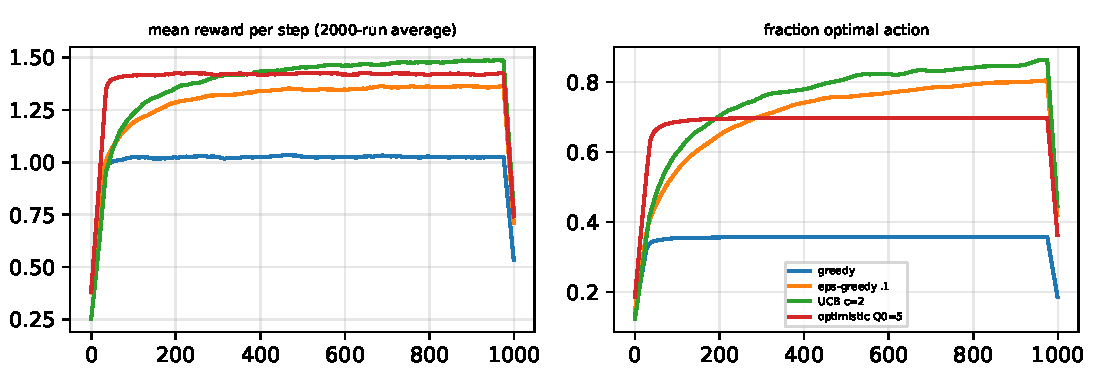
\includegraphics[width=\linewidth]{figures/ch13/bandit_curves.pdf}
\caption{2000-run averages (\texttt{code/ch13/bandits.py}): mean
reward per step (left) and fraction picking the optimal arm (right).
Greed plateaus early; UCB's calibrated optimism wins the long run.}
\label{fig:bandit}
\end{figure}

\section{MDPs: $(\mathcal S, \mathcal A, P, r, \gamma)$}
\label{sec:mdp}

A \textbf{Markov decision process}\index{MDP} formalises the loop:
states $\mathcal S$, actions $\mathcal A$, transition probabilities
$P(s' \mid s, a)$, reward function $r(s, a, s')$, discount
$\gamma \in [0, 1]$. ``Markov'' means the state must carry everything
the past could tell you --- the model's only structural demand. The
agent's goal is not the next reward but the \emph{discounted
return}\index{discounted return}:
\[
G_t = r_{t+1} + \gamma r_{t+2} + \gamma^2 r_{t+3} + \cdots
\]

\begin{example}[WE 13.2 --- $\gamma$ decides what the future costs]
\label{ex:gamma}
Take the reward sequence $[1,1,1,1,-3]$ --- four good steps, then a
crash (a policy that grabs quick rewards and dies). Figure~\ref{fig:discount}
computes $G_0$ at four discounts: $\gamma{=}0 \Rightarrow 1.00$ (the
myopic agent sees only the first 1, crash free);
$\gamma{=}0.5 \Rightarrow 1.69$; $\gamma{=}0.9 \Rightarrow 1.47$;
$\gamma{=}0.99 \Rightarrow 1.06$. Past $\gamma \approx 0.97$ the crash
outweighs all four gains and the policy should prefer a slower path.
Discounting is not a trick to make sums converge --- it is the
\emph{price of time}, and it changes which policy is optimal.
\end{example}

\begin{figure}[htbp]
\centering
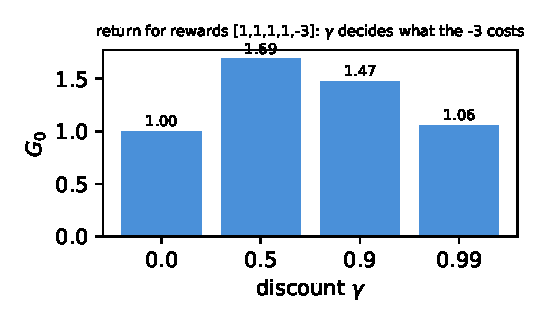
\includegraphics[width=0.62\linewidth]{figures/ch13/discount_returns.pdf}
\caption{$G_0$ for $[1,1,1,1,-3]$ as $\gamma$ varies: the same
behaviour is optimal under one discount and suicidal under another.}
\label{fig:discount}
\end{figure}

\section{Value functions and the Bellman equations}
\label{sec:bellman}

The \textbf{value function}\index{value function}
$V^\pi(s) = \mathbb E_\pi[G_t \mid s_t = s]$ answers ``how good is
this state under policy $\pi$''; the action-value
$Q^\pi(s,a)$ answers ``how good is this action, then following
$\pi$''. Both satisfy recursive \textbf{Bellman
equations}\index{Bellman equation}:
\[
V^\pi(s) = \sum_a \pi(a \mid s) \sum_{s'} P(s'\mid s,a)\,
\big[r + \gamma V^\pi(s')\big].
\]
Read it as bookkeeping: a state's value is the expected
immediate reward plus the discounted value of wherever you land.
Every algorithm in this chapter estimates this recursion --- the
differences are \emph{what they know} (a model vs samples) and
\emph{when they update} (episode end vs every step).

With a model, \emph{dynamic programming}\index{dynamic programming}
turns the equation into algorithms: \emph{policy evaluation} iterates
the Bellman equation until convergence; \emph{policy improvement}
acts greedily w.r.t.\ the result; alternating the two --- \emph{policy
iteration} --- reaches $\pi^*$ in finitely many rounds for small
MDPs, and \emph{value iteration} collapses both loops into one
contraction. DP is the theory; the next section is the practice.

\section{Model-free learning: MC, TD, Sarsa, Q-learning}
\label{sec:modelfree}

No model? Learn from the $(s,a,r,s')$ stream directly --- the
distinction is \emph{when} you update:

\begin{itemize}
\item \textbf{Monte Carlo}: run the episode, then update every
visited state toward the observed return $G_t$. Unbiased, slow to
react, works only on episodic tasks.
\item \textbf{TD(0)}\index{TD learning}: update \emph{each step}
toward a \emph{bootstrapped} target $r + \gamma V(s')$ --- learn a
guess from a guess. Biased early, lower variance, works online.
\item \textbf{Sarsa}: TD applied to $Q$: update $Q(s,a)$ toward
$r + \gamma Q(s', a')$ where $a'$ is what the agent \emph{actually
did} --- learns the value of the exploring policy (\emph{on-policy}).
\item \textbf{Q-learning}\index{Q-learning}: update toward
$r + \gamma \max_{a'} Q(s',a')$ --- the greedy action regardless of
what was done (\emph{off-policy}): it learns about the optimal policy
while behaving sloppily.
\end{itemize}

\begin{example}[WE 13.3 --- TD overtakes MC, on a 50-seed average]
\label{ex:mctd}
Figure~\ref{fig:mctd} is a real experiment, not an illustration: the
5-state random walk of Sutton \& Barto~\cite{suttonbarto2018}, each
method at its best $\alpha$, averaged over 50 seeds. At matched
$\alpha$ MC actually leads early; with each tuned fairly
(TD $\alpha{=}0.15$, MC $\alpha{=}0.03$) TD is ahead by episode 20 and
finishes at $0.074$ vs MC's $0.092$ RMS error. Bootstrapping reuses
every estimate as evidence --- the walk is tiny, but the mechanism
(bias-for-speed trade) is the one that runs inside every RL system
you will meet.
\end{example}

\begin{figure}[htbp]
\centering
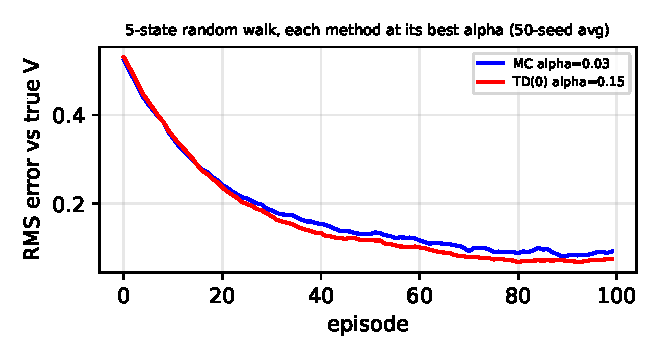
\includegraphics[width=0.72\linewidth]{figures/ch13/mc_vs_td_walk.pdf}
\caption{MC vs TD(0) on the random walk (50-seed average, each at its
best $\alpha$): TD's bootstrapped estimates converge lower --- the
honest version of the standard claim.}
\label{fig:mctd}
\end{figure}

\lstinputlisting[language=Python,caption={\texttt{code/ch13/qlearn\_grid.py}: tabular Q-learning on a FrozenLake-style $4\times4$ grid --- start, holes, goal --- with the learned greedy policy printed as moves.},label=lst:qlearn]{code/ch13/qlearn_grid.py}

\lstinputlisting[numbers=none]{code/ch13/qlearn_grid.out.txt}

\begin{example}[WE 13.4 --- Reading the learned Q-table]
\label{ex:grid}
The printed policy is a proof of learning, not a statistic: from
start the greedy run goes \texttt{D R D D R} --- around both holes,
into the goal, in 6 moves, return $0.93$ (six steps $\times$
$-0.01$ plus $+1$). Episodes 0--9 show the same agent falling into
holes ($-1.05, -1.45$) before the Q-table fills in; the last-100 mean
of $0.587$ lags the peak because $\varepsilon{=}0.15$ keeps spending
15\% of moves on exploration --- the bandit tax again, now with
states. Figure~\ref{fig:grid} draws the full $V^*$ field the table
converged to: the goal's $1.0$ bleeds backward through exactly the
cells a discount of $0.95$ predicts ($0.95$ one step out, $0.90$ two,
decaying toward the start's $0.83$).
\end{example}

\begin{figure}[htbp]
\centering
\begin{minipage}[t]{0.44\linewidth}
\centering
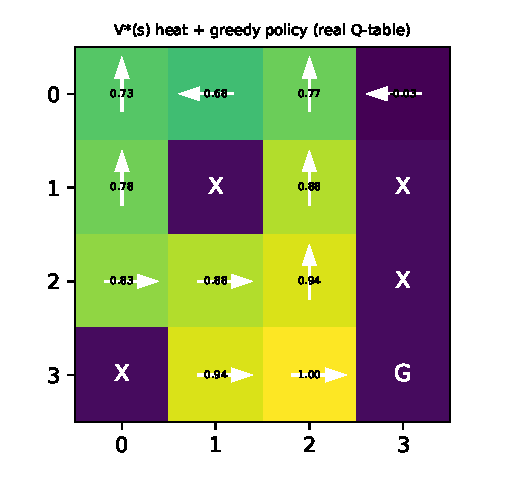
\includegraphics[width=\linewidth]{figures/ch13/gridworld_policy.pdf}
\caption{The real Q-table as a map: $V(s)$ heat and greedy policy.
The goal's value diffuses backward $\times 0.95$/step; holes are
voids the arrows route around.}
\label{fig:grid}
\end{minipage}\hfill
\begin{minipage}[t]{0.52\linewidth}
\centering
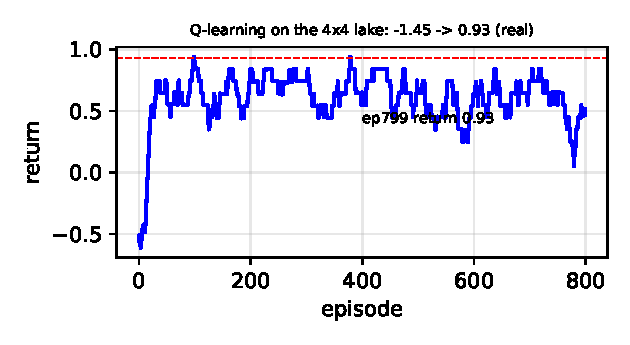
\includegraphics[width=\linewidth]{figures/ch13/qlearn_curve.pdf}
\caption{Return vs episode (\texttt{qlearn\_rews.npy}): falls into
holes, then solves it. The residual wobble is the fixed
$\varepsilon{=}0.15$ tax, not instability.}
\label{fig:qcurve}
\end{minipage}
\end{figure}

\section{Function approximation --- where the guarantee ends}
\label{sec:fa}

Tabular $Q$ dies when $|\mathcal S|$ explodes (CartPole's continuous
state, Go's $10^{170}$). The fix is to approximate $Q(s,a;\mathbf w)$
--- linear features, or a network --- and update $\mathbf w$ by TD
error. And here the guarantee ends: combining
\textbf{function approximation + bootstrapping + off-policy data} ---
the \emph{deadly triad}\index{deadly triad} --- can diverge
\cite{suttonbarto2018}. The next listing runs the failure live rather
than asserting it.

\lstinputlisting[language=Python,caption={\texttt{code/ch13/cartpole\_linear.py}: linear-function-approximation Q-learning on a hand-rolled CartPole (classic dynamics, no gym needed). It learns --- then unlearns. Keep the \texttt{|w|} column in sight.},label=lst:cartpole]{code/ch13/cartpole_linear.py}

\lstinputlisting[numbers=none]{code/ch13/cartpole_linear.out.txt}

\begin{example}[WE 13.5 --- It learned. Then it forgot: the triad, live]
\label{ex:triad}
Mean steps rise $41 \to 54$ over 200 episodes --- a real, if wobbly,
pole --- then collapse to $30$ by 400 while $|\mathbf w|$ balloons to
$4.35$. Nothing changed except the learner: the bootstrap target
$r + \gamma \max Q(s',a';\mathbf w)$ moves every step $\mathbf w$
moves, so the agent chases its own estimates; off-policy replay data
stops representing the current policy; and a linear $Q$ \emph{must}
misprice some states no matter what --- the errors land exactly where
the reward gradient points. The tabular gridworld had none of these
problems (exact representation, so targets eventually agree); the
CartPole run has all three, and this is the honest face of deep RL
engineering --- DQN's target networks and replay buffers exist
precisely to break the triad's coupling~\cite{spinningup}.
\end{example}

\begin{figure}[htbp]
\centering
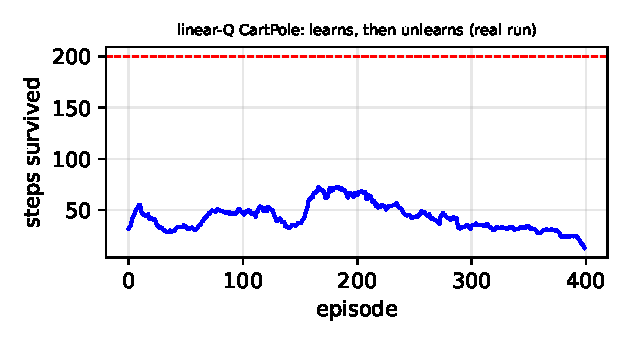
\includegraphics[width=0.72\linewidth]{figures/ch13/cartpole_fail.pdf}
\caption{Steps survived vs episode (\texttt{cartpole\_lens.npy}): the
rise is learning; the decay to $\sim$30 while weights grow is the
deadly triad, not a bug in the run.}
\label{fig:cartfail}
\end{figure}

\section{Policy gradient in one page}
\label{sec:pg}

Value methods learn \emph{what is good} then derive a policy; policy
gradients parameterise $\pi_\theta$ itself and push its parameters
along the reward gradient
$\nabla_\theta J = \mathbb E[G_t\,\nabla_\theta \log \pi_\theta(a_t
\mid s_t)]$ --- REINFORCE~\cite{williams1992}. No value table at all:
run the policy, weigh each action's log-probability by how well the
episode went, step. The variance is brutal without a learned baseline
(which is where actor--critic, PPO, and friends come from), but the
form is what matters here: it is exactly the update used to
\emph{post-train} language models --- sample completions, score them
with a reward signal (human preference, verifier, test suite), push
$\log \pi$ toward the scorers' favourites. Chapter 11's transformer
and this chapter's REINFORCE are the two halves of that story.

\section{Common mistakes}
\label{sec:rlmistakes}

\begin{description}
\item[Reward hacking] The agent optimises the reward, not the goal:
a shaping bonus for ``getting closer'' gets collected in circles; a
pole-balance that pays per-step gets gentle falling, not standing.
Your run prints what you asked for --- audit whether it is what you
meant~\cite{gymnasium_cartpole}.
\item[Reading return while $\varepsilon$ is fixed] Our gridworld's
$0.587$ mean vs $0.93$ greedy gap is exploration tax, not failure ---
evaluate greedy rollouts separately, or decay $\varepsilon$ on a
schedule before judging.
\item[Trusting a single run] Bandit rankings, CartPole collapses and
walk errors all swing between seeds; our claims ran at
2000-run/50-seed scale. One seed is an anecdote.
\item[Assuming function approximation inherits tabular guarantees]
It does not --- Example~\ref{ex:triad} is the honest version. Target
networks, replay buffers and smaller $\alpha$ are mitigations, not
theorems.
\item[Forgetting $\gamma$ changes the task] As WE~13.2 showed,
$\gamma{=}0$ and $\gamma{=}0.99$ are different problems; a ``bad''
agent is often a well-trained agent under a discount you did not
intend.
\item[Treating the world as IID] The agent's own policy decides which
states it sees --- coverage collapses just like the GAN's did in
ch12, silently.
\end{description}

\section{Summary table}
\label{sec:rlsummary}

\begin{center}\small
\begin{tabular}{p{2.4cm}p{3.0cm}p{2.6cm}p{2.6cm}p{2.2cm}}
\toprule
method & needs & updates at & guarantee & our number \\
\midrule
$\varepsilon$-greedy bandit & rewards only & each step & regret bound (loose) & 1.362 (80\% opt) \\
UCB bandit & rewards only & each step & near-optimal regret & 1.482 (86\% opt) \\
policy/value iteration & full model & sweep & exact $\pi^*$ (small MDPs) & --- (theory) \\
MC & episodes & episode end & unbiased, slow & RMS 0.092 \\
TD(0)/Sarsa & $(s,a,r,s')$ & each step & on-policy value & RMS 0.074 \\
Q-learning & $(s,a,r,s')$ & each step & tabular $\to Q^*$ & 0.93 return \\
linear FA + Q & features & each step & \textbf{none} (triad) & 30 steps collapse \\
\bottomrule
\end{tabular}
\end{center}

The ladder: know nothing (bandit), know the model (DP), know only
experience (MC/TD/Q), approximate (FA) --- each rung trades guarantees
for reach. Policy gradient skips the value function entirely and pays
for it in variance; everything in modern RL is a way to buy some of
it back.

\section*{Drill}
\begin{enumerate}
\item What problem exists in a bandit that does not exist in
supervised learning --- and what does UCB add to $\varepsilon$-greedy's
answer?
\item Compute $G_0$ for rewards $[2,-1,3]$ at $\gamma{=}0.9$.
\item State the Bellman equation for $V^\pi$ in words.
\item Sarsa vs Q-learning: which term of the update differs, and why
does that make one on-policy and one off-policy?
\item Name the three ingredients of the deadly triad.
\end{enumerate}

\section*{Further reading}
\label{sec:further13}
\begin{itemize}
\item Sutton \& Barto, \emph{Reinforcement Learning: An Introduction}
(2nd ed.) --- the book; our bandit, random-walk and Q-learning numbers
are its chapters 2, 6, 7 run locally.
\url{https://web.stanford.edu/class/psych209/Readings/SuttonBartoIPRLBook2ndEd.pdf}
\item OpenAI, \emph{Spinning Up in Deep RL} --- the engineering bridge
from this chapter to DQN/PPO, with the triad fixes spelled out.
\url{https://spinningup.openai.com/en/latest/}
\item D.~Silver, \emph{RL course} --- the UCL lectures the field was
trained on; lecture notes and slides.
\url{https://www.davidsilver.uk/teaching/}
\item Williams, \emph{Simple statistical gradient-following
algorithms} (1992) --- REINFORCE, the update behind \S\ref{sec:pg}
and LLM post-training.
\url{https://papers.nips.cc/paper_files/paper/1999/hash/464d828b85b0bed98e80ade0a5c43b0f-Abstract.html}
\item Gymnasium, \emph{Cart Pole} --- the environment spec our
physics implements.
\url{https://gymnasium.farama.org/environments/classic_control/cart_pole/}
\item Hugging Face, \emph{Deep RL Course} --- a free modern course
from this chapter's topics onward.
\url{https://huggingface.co/learn/deep-rl-course/en/unit0/introduction}
\item Wikipedia, \emph{Q-learning} --- convergence conditions and
history, well cross-linked. \url{https://en.wikipedia.org/wiki/Q-learning}
\end{itemize}

\begin{rulebox}[Watch instead]
(verified opened, 2026-10-11)
\begin{itemize}
\item \emph{Introduction to Reinforcement Learning} --- David Silver,
RL Course Lecture 1 (88:12). The whole framing of this chapter:
agent, reward, MDP, value.
\item \emph{Deep Reinforcement Learning} --- Stanford Engineering
Lecture 14 (64:01). Where value methods meet the function
approximation that broke our CartPole.
\end{itemize}
\end{rulebox}

\section*{Notes}
\begin{enumerate}
\item[\textbf{1.}] All runs are real and local: bandits averaged over
2000 independent runs (S\&B protocol), the gridworld trained 800
episodes at $\alpha{=}0.6, \gamma{=}0.95, \varepsilon{=}0.15$,
CartPole ran 400 episodes of hand-implemented classic dynamics
($\tau{=}0.02$, forces $\pm10$) --- no gymnasium dependency needed.
\item[\textbf{2.}] The MC-vs-TD figure uses the fair-comparison
convention (each method at its best $\alpha$, 50-seed average);
at matched $\alpha$ the early-episode order reverses, which is why
the caption and Example~\ref{ex:mctd} say ``overtakes'' rather than
``wins''.
\item[\textbf{3.}] The CartPole divergence is deliberately uncorrected:
fixing it is what target networks, replay buffers and Double-Q exist
for, and they belong to the deep-RL literature~\cite{spinningup},
not this chapter.
\item[\textbf{4.}] Deliberately out of scope: eligibility traces,
Double/dueling/rainbow architectures, model-based planning
(Dyna, MCTS), offline and safe RL, and the full PPO/RLHF machinery
--- \S\ref{sec:pg} gives the seed of the last one only.
\item[\textbf{5.}] The canonical Sutton \& Barto site
(incompletedideas.net) was unreachable at verification time; the
Stanford-hosted PDF of the same edition is cited instead and the
original is logged as [unverified] in \texttt{docs/}\allowbreak\texttt{unverified.md}.
\end{enumerate}

\section{Exercises}
\label{sec:rlex}

\emph{[easy]}
\begin{exercise}
Compute $G_0$ for rewards $[2,-1,3]$ at $\gamma{=}0.9$, then at
$\gamma{=}0$. Which policy would each prefer: take the -1 hit now for
the 3, or stop after the first 2?
\end{exercise}
\begin{exercise}
Write the Bellman equation for $Q^\pi(s,a)$ mirroring the one for
$V^\pi(s)$ in \S\ref{sec:bellman}.
\end{exercise}
\begin{exercise}
In our gridworld, the goal cell's $V$ is 1.0 and $\gamma{=}0.95$.
What is $V$ of the cell two moves away? Why is the start cell's $V$
lower than $0.95^5$?
\end{exercise}
\begin{exercise}
Our bandit run prints $80\%$ optimal-arm for $\varepsilon$-greedy,
not $100\%$. Two distinct reasons --- name them.
\end{exercise}

\emph{[medium]}
\begin{exercise}
Implement UCB yourself: modify \texttt{bandits.py} so the bonus is
$c\sqrt{\ln t / N_a}$ with $c \in \{0.5, 2, 8\}$. Report
mean-reward(1000) for each and explain the $c{=}8$ result.
\end{exercise}
\begin{exercise}
Write value iteration for the $4\times4$ grid (with the model, not
samples): $V(s) \leftarrow \max_a \sum_{s'} P[r+\gamma V(s')]$.
How many sweeps until the greedy policy matches our learned Q-table's?
\end{exercise}
\begin{exercise}
Change \texttt{qlearn\_grid.py} to decay
$\varepsilon \leftarrow 0.5 \cdot 0.995^{\mathrm{ep}}$. Re-run and
report the last-100 mean: how much of the 0.587 gap was exploration
tax?
\end{exercise}
\begin{exercise}
Convert \texttt{qlearn\_grid.py} to Sarsa (update with the action
actually taken). Run both on the grid and explain any difference in
the learned policy near the holes.
\end{exercise}
\begin{exercise}
In \texttt{cartpole\_linear.py}, lower the learning rate to
$0.002$ and add a target $Q$ frozen every 20 episodes. Does the
|w|-blowup move, and by how much? Report the numbers.
\end{exercise}
\begin{exercise}
Our reward gives $-0.01$/step. Re-run the gridworld at $-0.05$/step
and at $0$/step: at which value does the learned policy change, and
why?
\end{exercise}

\emph{[hard]}
\begin{exercise}
Prove the greedy-policy improvement lemma: if $\pi'$ acts greedily
w.r.t.\ $Q^\pi$, then $V^{\pi'}(s) \geq V^\pi(s)$ for all $s$.
\end{exercise}
\begin{exercise}
Derive the TD(0) update as a bootstrapped sample of the Bellman
equation: start from $V(s) = \mathbb E[r + \gamma V(s')]$, replace the
expectation by one sample, and write the resulting update. Where does
the bias live?
\end{exercise}
\begin{exercise}
Maximisation bias: $\max_a Q(s,a)$ overestimates $\max_a Q^*(s,a)$
whenever estimates are noisy --- our gridworld's early episodes
show it. Implement Double-Q (two tables, update one, evaluate with
the other) on the $4\times4$ grid and measure how the early-return
curve changes.
\end{exercise}
\begin{exercise}
The REINFORCE estimator
$\mathbb E[G_t \nabla_\theta \log \pi_\theta(a_t\mid s_t)]$ has huge
variance. Show that subtracting any state-dependent baseline
$b(s_t)$ leaves the expectation unchanged, and argue why
$b = V(s)$ is the best cheap choice.
\end{exercise}
\begin{exercise}
Design (do not run) the reward-hacking audit for our CartPole:
which three measurements would tell you the agent maximises
reward without balancing --- and which of them does our failure
already print?
\end{exercise}

\section*{Hints and answers}
\begin{description}
\item[1.] $2 + 0.9(-1) + 0.81(3) = 3.53$ vs $2$ at $\gamma{=}0$ ---
the patient policy takes the hit.
\item[2.] $Q^\pi(s,a) = \sum_{s'} P[r + \gamma \sum_{a'} \pi(a'\mid s')
Q^\pi(s',a')]$.
\item[3.] $0.95^2 = 0.90$; start is lower because episodes can die in
holes on the way --- $V$ counts risk, not just distance.
\item[4.] $\varepsilon$-greedy explores forever (10\% random), and
80\% is measured \emph{while} exploring --- the greedy choice alone
is higher.
\item[5.] $c{=}0.5$ under-explores; $c{=}8$ over-pays for information
--- the bonus dominates $Q$ so long it behaves like a random walker
with a preference.
\item[6.] Usually 2--4 sweeps on this grid --- the value field
diffuses one cell per sweep.
\item[7.] Expect $\approx 0.85$--$0.93$: most of the $0.93-0.587$ gap
is the 15\% tax, the rest is leftover uncertainty.
\item[8.] Sarsa's policy hugs safe routes (it learns what the
exploring agent would do); Q-learning is braver --- it prices the
greedy future.
\item[9.] The blowup slows but the late-episode decay stays --- the
mitigation delays the triad, it does not repeal it.
\item[10.] At $0$/step the policy still reaches the goal but stops
hating detours --- the $-0.01$ is the shortest-path pressure.
\item[11.] Expand $V^{\pi'}(s) \geq \mathbb E_{\pi'}[r + \gamma
V^\pi(s')]$ and iterate --- each expansion replaces $V^\pi$ with the
larger greedy target.
\item[12.] The bias lives in $V(s')$ itself --- the estimate you
bootstrap from is wrong until everything else converges.
\item[13.] Double-Q decouples selection from evaluation; expect
smaller early returns, less overconfidence in the printed table.
\item[14.] $\mathbb E[b(s)\nabla\log\pi] = b(s)\nabla\sum_a\pi = 0$;
$V(s)$ is the mean return's best estimator, so it removes the
part of $G_t$ the state predicts.
\item[15.] Step counts, pole-angle traces, and action entropy --- the
angle trace and |w|-growth already print in this chapter's run.
\end{description}
